\documentclass[ucs, notheorems, handout]{beamer}
	
\usefonttheme[onlymath]{serif}
\setbeamertemplate{navigation symbols}{}

	
\usepackage[utf8x]{inputenc}
\usepackage[T2A]{fontenc}
\usepackage[russian]{babel}
\usepackage{tikz}
\usepackage{ragged2e}
\usepackage{amsthm}
\usepackage{wrapfig}
\usepackage{bm} %bold math
\usepackage{url}	
\usepackage{graphicx}
\usepackage{marginnote}
\usepackage{bm}
\usepackage[makeroom]{cancel}
\usepackage{algorithm2e}
\newcommand{\sign}{\text{sign}}
\DeclareMathOperator*{\argmax}{arg\,max}
\DeclareMathOperator*{\argmin}{arg\,min}
\DeclareMathOperator{\rank}{rank}
\DeclareMathOperator{\diam}{diam}
\DeclareMathOperator{\ob}{Ob}
\DeclareMathOperator{\Hom}{Hom}
\DeclareMathOperator{\var}{Var}
\DeclareMathOperator{\bias}{Bias}
\newcommand{\betah}{\hat{\bm \beta}}
\newcommand{\betaa}{\bm{\beta}}
\newcommand{\epss}{\bm{\varepsilon}}
\newcommand{\E}{\mathrm{E}}
\newcommand{\D}{\mathrm{D}}
\newcommand{\XT}{{\bm{X}}^{\mathrm{T}}}
\newcommand{\X}{\bm{X}}
\renewcommand{\thealgocf}{}
\definecolor{asparagus}{rgb}{0.53, 0.66, 0.42}
	
\newtheorem{theorem}{Теорема}
\newtheorem{definition}{Определение}
\addto\captionsrussian{\renewcommand{\figurename}{Figure}}
\addto\captionsrussian{\renewcommand{\tablename}{Table}}
	
\title[Обучение без учителя. Разделение смеси распределений. Кластеризация. Тематическое обучение (Probabilistic LSA)]{%
	    Обучение без учителя. Разделение смеси распределений. Кластеризация. Тематическое обучение (Probabilistic LSA)}
	
\author[Михайлов Дмитрий, Cмирнов Иван]{Михайлов Дмитрий, Cмирнов Иван}
	
\institute[Санкт-Петербургский Государственный Университет]{%
	    \small
	    Санкт-Петербургский государственный университет\\
	    Кафедра статистического моделирования\\
	    \vspace{1.25cm}
	}
	
\date[]{Санкт-Петербург, 2023}
	
%\subject{Talks}
	
\begin{document}
	
	\begin{frame}[plain]
		\titlepage
	\end{frame}
	
	
	\begin{frame}
	\frametitle{Обучение без учителя}
		Обучение без учителя - это один из способов машинного обучения, при котором испытуемая система обучается выполнять поставленную задачу без вмешательства со стороны экспериментатора.  Как правило, это пригодно только для задач, в которых известны описания множества объектов (обучающей выборки), и требуется обнаружить внутренние взаимосвязи, зависимости, закономерности, существующие между объектами.
	
		Обучение без учителя становится формально поставленной задачей только в случае, если можно написать функцию правдоподобия.
		\vspace{0.5cm}  
	\end{frame}
	
	\begin{frame}
	\frametitle{Кластеризация. Введение}
		Задача кластеризации заключается в том чтобы выполнить разбиение индивидов на кластеры на основе их сходства друг с другом (близость относительно выбранной метрики), при этом сами кластеры или их количество, как правило, заранее не известны. Кластеры строятся так, что характеристики для объектов внутри одного кластера близки, а характеристик объектов из разных кластеров сильно отличаются.
		\vspace{0.5cm}  
	\end{frame}
	
	\begin{frame}
	\frametitle{Кластеризация. Формальное описание задачи}
		Пусть имеется подмножество $\pmb X \subset \mathbb{R}^{p}$, которое будем называть
пространством объектов, выборка $\pmb X^{n} = \{\pmb x_1, \dots, \pmb x_{n}\}$, где $\pmb x_{i} $ --- индивиды, определяемые вектором признаков, $C$ --- множество кластеров. Задача состоит в том чтобы найти такую функцию $a: X \rightarrow Y$, которая разбила бы выборку на непересекающиеся кластеры $\pmb X^{n}= \bigcup_{j = 1}^{k} C_{j}, \  C_{i} \bigcap C_{j} = \emptyset$, таким образом, чтобы объекты одного кластера были близки по функции расстояния между объектами $\rho :  \mathbb{R}^{p} \times  \mathbb{R}^{p} \rightarrow [0,\infty)$ и существенно отличались для объектов разных кластеров.
		\vspace{0.5cm}  
	\end{frame}
	
	\begin{frame}
	\frametitle{Кластеризация. Формальное описание задачи}
		Не существует <<истинных>> или <<лучших>> определений для кластера. Что понимать под кластером должно быть определено исследователем, который применяет методы кластеризации. Как правило, для этого нужно определить характеристики кластера в отношении размера и формы, а также предполагаемых различий между кластерами.

		Общая схема процесса кластеризации данных включает в себя: 
		\begin{itemize}
			\item определение меры сходства;
			\item разбиение множества объектов на кластеры;
			\item оценку качества кластеризации;
			\item интерпретацию результатов.
		\end{itemize}
	
		Решение задачи кластеризации принципиально неоднозначно, так как число кластеров, как правило, не известно заранее, к тому же результат кластеризации сильно зависит от метрики $\rho$, выбор которой также не однозначен.
 
	\end{frame}
	
	\begin{frame}
	\frametitle{Кластеризация. EM - алгоритм для model-based подхода}
		Один из вариантов формализовать задачу кластеризации это сделать предположение о статистическом распределении данных. Затем задача будет состоять в поиске параметров этого распределения. Предположим, что модель данных состоит из $k$ смеси распределений. Пусть $\omega_{1}\ldots \omega_{k}$ --- априорные вероятности появления объектов из соответствующих кластеров, $p_{1}(x)\ldots p_{k}(x)$ --- плотности распределения признаков внутри кластеров. Тогда плотность распределения сразу для всех кластеров равна взвешенной сумме плотностей по каждому кластеру:
		$$
		p(x) = \sum\limits_{i=1}^k \omega_{i} p_{i}(x).
		$$
 
	\end{frame}
	
	\begin{frame}
	\frametitle{Кластеризация. EM - алгоритм для model-based подхода}
		
		Поставим задачу разделения смеси распределений, оценим по выборке $\omega_{1}\ldots \omega_{k}$ и $p_{1}(x)\ldots p_{k}(x)$. Это позволит оценить вероятность принадлежности индивида к разным кластерам и решить к какому кластеру его отнести. Часто рассматриваются случаи когда распределение смеси принадлежат одному семейству распределений, например нормальному, но с разным набором параметров для каждого из кластеров. 
		$$
		p_{i}(x) = \varphi(\theta_{i}; x)
		$$
		Согласно методу максимального правдоподобия 
		$$
		\omega, \theta = \underset{\omega, \theta}{\text{argmax}} \sum\limits_{i=1}^n \ln{p(x_{i})}  =  \underset{\omega, \theta}{\text{argmax}} \sum\limits_{i=1}^n \ln  \sum\limits_{j=1}^k \omega_{j}  \varphi(\theta_{j}; x_{i})
		$$
		Максимизация логарифма суммы достаточно сложна, поэтому задача не решается напрямую с помощью метода максимума правдоподобия. Для максимизации логарифма функции правдоподобия применяется EM-алгоритм.
	\end{frame}
	
	\begin{frame}
	\frametitle{Кластеризация. EM - алгоритм для model-based подхода}
		
		\textbf{E - шаг.}
		
		В начале работы алгоритма задаём значения параметров $\omega, \theta = (\omega_{1}\ldots, \omega_{k};\theta_{1}\ldots \theta_{k})$, и подставляя их рассчитываем скрытые переменные. Скрытые переменные $h_{ij} = P(\theta_{j}|x_{i})$ --- это вероятность того, что индивид $x_{i}$ принадлежит $j$ смеси. Найдем скрытые переменные по формуле Байеса:
		$$
		h_{ij} = \frac{ \omega_{j} \varphi(\theta_{j}; x_{i})}{\sum\limits_{s=1}^k \omega_{s}  \varphi(\theta_{s}; x_{i})}.
		$$
		Для любого индивида $\sum\limits_{j=1}^k h_{ij} = 1.$
	\end{frame}
	
	\begin{frame}
	\frametitle{Кластеризация. EM - алгоритм для model-based подхода}
		
		\textbf{M - шаг.}

		На этом шаге будут рассчитываться значения параметров, которые мы ищем, используя скрытые параметры, полученные на предыдущем шаге. Решение методом Лагрнажа для максимизации логарифма правдоподобия (c ограничением $\sum\limits_{j=1}^k\omega_{j}=~1$) даёт оценку для параметров:
		$$
		\omega_{j} = \frac{1}{n} \sum\limits_{i=1}^n h_{ij}
		$$
		$$
		\theta_{j} = \underset{\theta}{\text{argmax}} \sum\limits_{i=1}^n h_{ij} \ln{\varphi(\theta; x_{i})}
		$$
		Таким образом, параметры будут уточняться на каждом шаге.
	\end{frame}
	
	\begin{frame}
	\frametitle{Кластеризация. EM - алгоритм для model-based подхода}
		Если сделать предположение о том что классы принадлежат семейству нормальных распределений, то параметрами модели являются математическое ожидание и ковариационная матрица. Если не делать никаких предположений о ковариациях использование общей модели может быть весьма затруднительно, проблема заключается в большом количестве параметров, которые необходимо оценить. Ковариационные матрицы описывают геометрические характеристики кластеров, а именно объем, форму и ориентацию кластера. Общая модель предполагает, что все эти геометрические характеристики различны для каждого кластера. Однако, оценка плотности смеси, состоящей из кластеров одинаковой формы или ориентации, намного проще. Поэтому, сделав предположения о ковариационных матрицах, можно существенно облегчить задачу.
	\end{frame}
	
	\begin{frame}
	\frametitle{Кластеризация. Алгоритм k-средних (k-means)}
		Метод k-means осуществляет декомпозицию набора данных, состоящего из $n$ наблюдений, на $k$ кластеров с заранее неизвестными параметрами. При этом выполняется поиск центроидов - максимально удаленных друг от друга центров сгущений точек $C_k$ с минимальным разбросом внутри каждого кластера. 
	
		В качестве меры близости выбрано евклидово расстояние: $$ d(\pmb x_{i}, \pmb x_{i'}) = \sum\limits_{j=1}^p (x_{ij} - x_{i'j})^{2} = \| \pmb x_{i} - \pmb x_{i'} \|^{2}. $$
		
		Основная идея алгоритма заключается в минимизации меры близости между индивидами внутри одного кластера: $$ \underset{C_{1},\ldots, C_{k}}\min \left\{ \sum\limits_{l=1}^k \frac{1}{|C_{l}|} \sum\limits_{i,i' \in C_{l}} \| \pmb x_{i} - \pmb x_{i'} \|^{2} \right\}. $$
	\end{frame}
	
	\begin{frame}
	\frametitle{Кластеризация. Алгоритм k-средних (k-means)}
		\begin{enumerate}
		\item Выбираем начальное приближение центров кластеров $\pmb \mu_{1},\ldots, \pmb \mu_{k}$ случайным образом; 
		\item Соотносим каждый объект к ближайшему центру (аналог E-шага) $$C(i) = \underset{0 \leq j \leq k}{\text{argmin}} \|\pmb x_{i} - \pmb \mu_{j} \|^{2};$$
		\item Для каждого кластера $C_{j}$ пересчитываем центры $\pmb \mu_{j}$ как выборочное среднее индивидов, которые были отнесены к этому кластеру (аналог M-шага);
		\item  Повторяем шаги 2 и 3 пока принадлежность кластерам не перестанет изменяться.
	\end{enumerate}
		
		Иными словами, делаем следующее: инициализируем центры, затем разделяем индивиды по ближайшему центру кластера, перевычисляем каждый из центров, и если ничего не изменилось, останавливаемся, если изменилось, то повторяем.
	\end{frame}
	
	\begin{frame}
	\frametitle{Кластеризация. Алгоритм k-средних (k-means)}
			\textbf{Достоинства:}
		\begin{itemize} 
			\item Простота реализации
			\item Алгоритм очень гибкий 
			\item Cуществует множество различных модификаций этого алгоритма
		\end{itemize}
		
		\textbf{Недостатки:} 
		\begin{itemize}
			\item Кластеризация очень сильно зависит от начального приближения\\
			\item Кластеризация может быть неадекватной, если изначально было выбрано неверное число кластеров 
			\item Необходимость самостоятельно задавать число кластеров\\ 
			\item Форма кластеров только сферическая
		\end{itemize}

	\end{frame}
	
	\begin{frame}
	\frametitle{Кластеризация. Иерархическая кластеризация}
		Методы иерархической кластеризации основываются на двух идеях:
	\begin{itemize}
		\item агломерации (AGNES) --- последовательное объединение индивидуальных объектов или их групп во все более крупные подмножества
		\item разбиении (DIANA) ---  начинается с корня и на каждом шаге делит образующие группы по степени их гетерогенности
	\end{itemize}

	Более распространены агломеративные алгоритмы, общий вид которых приведён дальше. 

	\end{frame}
	
	\begin{frame}
	\frametitle{Кластеризация. Иерархическая кластеризация}
			\begin{enumerate}
			\item Одноэлементые кластеры: $$C_1 = \left\{\{\pmb x_1\}, \dots, \{\pmb x_n\}\right\}; \; R_1 = 0$$ $$\forall\, i \neq j \text{ вычислить } R(\{\pmb x_i\}, \{\pmb x_j\})$$ 
			\item для всех $t = 2, \dots, n$ ($t$ $-$ номер итерации) 
			\item найти в $C_{t-1}$ два ближайших кластера: $$(U, V) = \arg \min_{U \neq V} R(U, V); R_t=R(U, V);$$
			\item слить их в один кластер: $$W = U \cup V; \; C_t = C_{t-1} \cup W \backslash \{U, V\}$$ 
			\item для всех $S \in C_t \backslash W $ 
			\item вычислить расстояние $R(W, S)$ по формуле Ланса-Уильямса.
			\end{enumerate}


	\end{frame}
	
	\begin{frame}
	\frametitle{Кластеризация. Иерархическая кластеризация}
	
		В начальный момент времени каждый объект содержится в собственном кластере. Далее происходит итеративный процесс слияния двух ближайших кластеров до тех пор, пока все кластеры не объединятся в один или не будет найдено необходимое число кластеров. На каждом шаге необходимо уметь вычислять расстояние между кластерами и пересчитывать расстояние между новыми кластерами. 

	\end{frame}
	
	\begin{frame}
	\frametitle{Кластеризация. Иерархическая кластеризация}
	
	Расстояние между одноэлементными кластерами определяется через расстояние между объектами: $R(\{x\}, \{y\})= \rho(x,y)$. То есть сначала нужно задать, как мы будем измерять расстояние между точками. Например, это могут быть
\begin{itemize}
	\item Евклидово расстояние: $\rho(x,y) = \sqrt{\sum_i (x_i - y_i)^2}$.
	\item Расстояние городских кварталов (манхэттенское расстояние):  $\rho(x,y) = \sum_i |x_i - y_i|$.
	\item Расстояние Чебышёва: $\rho(x,y) = \max_i |x_i - y_i|$.
\end{itemize}
Важно либо исходно стандартизовать признаки, либо измерять расстояние
специальным образом (использовать расстояние Махаланобиса вместо обычного евклидового, если есть предположения о форме распределения точек внутри кластера).
	\end{frame}
	
	\begin{frame}
	\frametitle{Кластеризация. Иерархическая кластеризация}
	
	Для вычисления же расстояния $R(U, V)$ между кластерами $U$ и $V$ на практике используются различные функции в зависимости от специфики задачи.
Изначально было придумано множество различных способов определить такие расстояния, но оказалось, что практически все разумные, являются частным случаем \textbf{формулы Ланса-Уильямса}, которая позволяет обобщить большинство способов определить расстояние между кластерами $ R(W, S),\; W = U \cup V,\, U,\, V,\, S \subset X, $ зная расстояния $R(U, S)$, $R(V, S)$, $R(U, V)$: 
	
	$$ R(W, S) = \alpha_{U} R(U, S) + \alpha_{V} R(V, S) + \beta R(U, V) + \gamma|R(U, S) - R(V, S)|,$$
	
	где $\alpha_{U}$, $\alpha_{V}$, $\beta$, $\gamma$ --- числовые параметры.
	\end{frame}
	
	\begin{frame}
	\frametitle{Кластеризация. Иерархическая кластеризация}
	
	Ниже приведены некоторые способы определения расстояний явно и соответствующие им коэффициенты для формулы Ланса-Уильямса. 
\begin{itemize}
	\item Расстояние ближнего соседа (single linkage clustering) --- расстояние между кластерами оценивается как минимальное из дистанций между парами объектов, один из которых входит в первый кластер, а другой - во второй:
	$$R^{\text{б}}(W, S) = \min_{w \in W, s \in S} \rho(w, s); \quad \alpha_U=\alpha_V=1/2,\enspace \beta=0,\enspace \gamma=-1/2;$$
	\item Расстояние дальнего соседа (complete linkage clustering) --- вычисляется расстояние между наиболее удаленными объектами:
	$$R^{\text{д}}(W, S) = \max_{w \in W, s \in S} \rho(w, s); \quad \alpha_U=\alpha_V=1/2,\enspace \beta=0,\enspace \gamma=1/2;$$
\end{itemize}.
	\end{frame}
	
	\begin{frame}
	\frametitle{Кластеризация. Иерархическая кластеризация}
	
\begin{itemize}
	
	\item Среднее расстояние (average linkage clustering) --- на каждом следующем шаге объединяются два ближайших кластера, рассчитывая среднюю арифметическую дистанцию между всеми парами объектов:
	$$R^{\text{с}}(W, S) = \frac{1}{ |W| |S| } \sum_{w \in W} \sum_{s \in S} \rho(w, s); \quad $$ $$ \alpha_U=\frac{|U|}{|W|},\enspace \alpha_V=\frac{|V|}{|W|},\enspace \beta=\gamma=0;$$
	
	\item Расстояние между центрами:
	$$R^{\text{ц}}(W, S) = \rho^2 \left( \sum_{w \in W} \frac{w}{|W|}, \sum_{s \in S} \frac{s}{|S|}\right); \quad
	$$ $$\alpha_U=\frac{|U|}{|W|},\enspace \alpha_V=\frac{|V|}{|W|},\enspace \beta= -\alpha_U \,\alpha_V,\enspace \gamma=0;$$
	
\end{itemize}.
	\end{frame}
	
	\begin{frame}
	\frametitle{Кластеризация. Иерархическая кластеризация}
	
\begin{itemize}
	\item Расстояние Уорда (метод минимума дисперсии Уорда):
	$$R^{\text{ц}}(W, S) = \frac{|S| |W|}{|S| + |W|} \rho^2 \left( \sum_{w \in W} \frac{w}{|W|}, \sum_{s \in S} \frac{s}{|S|}\right);$$  
	$$\alpha_U=\frac{|S|+|U|}{|S|+|W|},\enspace \alpha_V=\frac{|S|+|V|}{|S|+|W|},\enspace \beta= -\frac{|S|}{|S|+|W|},\enspace \gamma=0;$$
	
	\item Гибкое расстояние: $$\scalebox{0.9}{$\alpha_U=\alpha_V=\frac{1-\beta}{2},\enspace \beta<1 \;(-0.25),\enspace \gamma=0$}.$$
\end{itemize}.
	\end{frame}
	
	\begin{frame}
	\frametitle{Кластеризация. Иерархическая кластеризация}
	Результатом работы иерархического алгоритма является \textbf{дендрограмма} 
--- древовидный график расстояний, при которых произошло слияние кластеров на каждом шаге.
\begin{figure}[H]
	\centering
	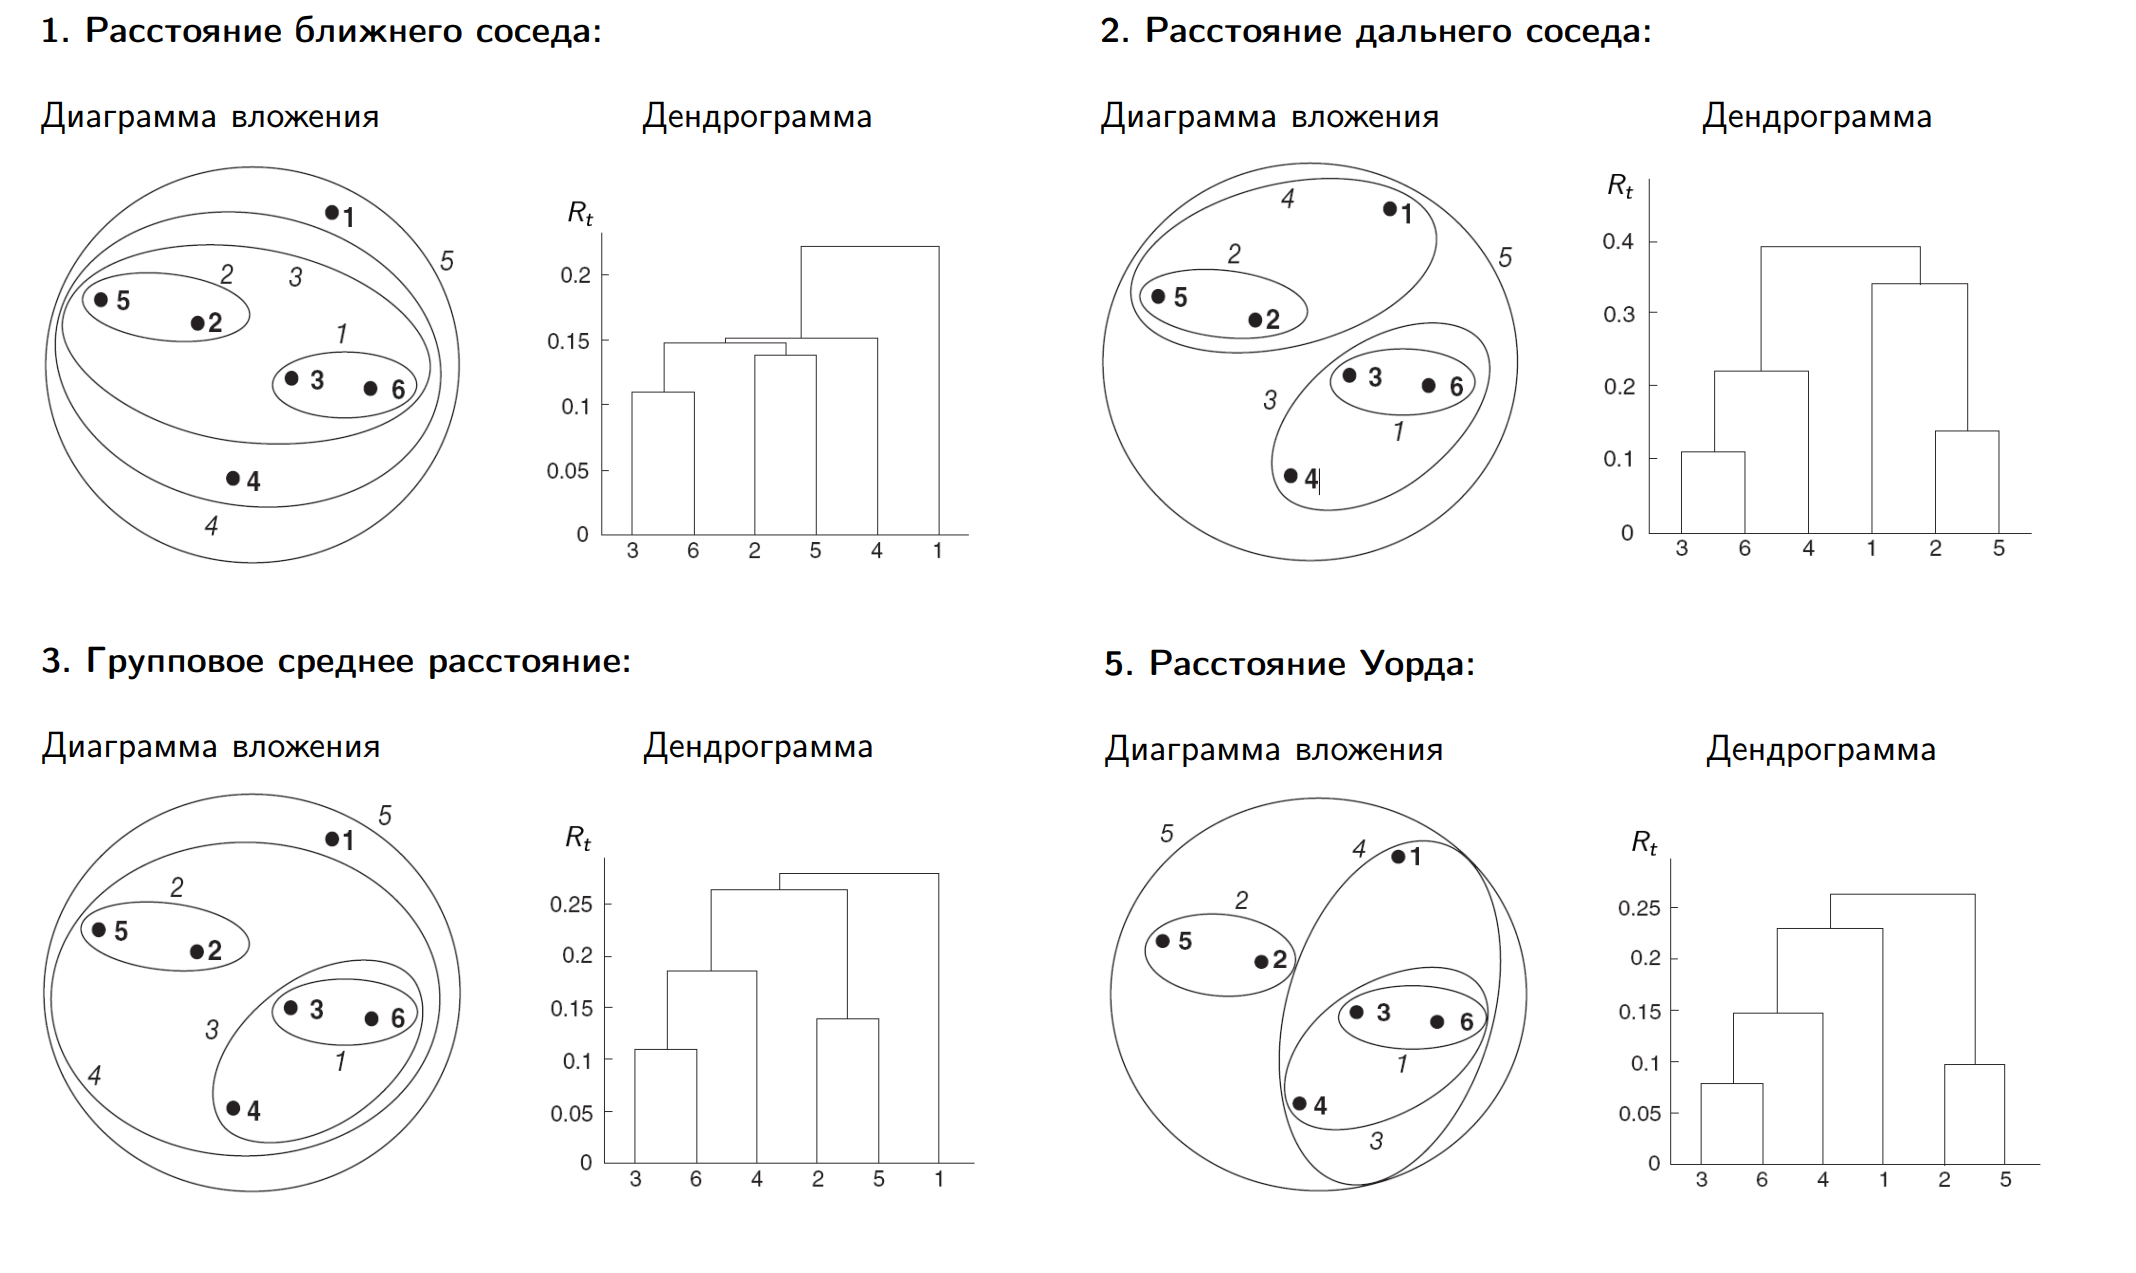
\includegraphics[scale=0.15]{hier.png}
	\caption{Дендрограммы при выборе различных расстояний.}
\end{figure}
	\end{frame}
	
	\begin{frame}
	\frametitle{Кластеризация. Алгоритм DBSCAN}
	\textbf{DBSCAN} (Density-based spatial clustering of applications with noise) --- это эвристический алгоритм кластеризации, который предложили Маритин Эстер, Ганс-Петер Кригель, Ёрг Сандер и Сяовэй Су в 1996. Это алгоритм кластеризации, основанный на плотности --- алгоритм группирует вместе те объекты, которые тесно расположены, помечая как выбросы объекты, которые находятся в областях с малой плотностью.

	
В этом алгоритме рассматривается для каждого объекта $\pmb x \in U$ его $\varepsilon$-окрестность $U_\varepsilon (\pmb x) = \{\pmb u \in U : \rho(\pmb x , \pmb u ) \leq \varepsilon\}$.
	\end{frame}
	
	\begin{frame}
	\frametitle{Кластеризация. Алгоритм DBSCAN}
	В этом алгоритме рассматривается для каждого объекта $\pmb x \in U$ его $\varepsilon$-окрестность $U_\varepsilon (\pmb x) = \{\pmb u \in U : \rho(\pmb x , \pmb u ) \leq \varepsilon\}$.
	
Каждый объект может быть одного из трёх типов:
	\begin{itemize}
		\item корневой: имеет плотную окрестность $|U_\varepsilon (\pmb x)| \geq m$ 
		\item граничный: не корневой, но находится в окрестности корневого 
		\item выброс: не корневой и не граничный. 
	\end{itemize}
	\end{frame}
	
	\begin{frame}
	\frametitle{Кластеризация. Алгоритм DBSCAN}
	
	\begin{figure}[H]
		\begin{center}
			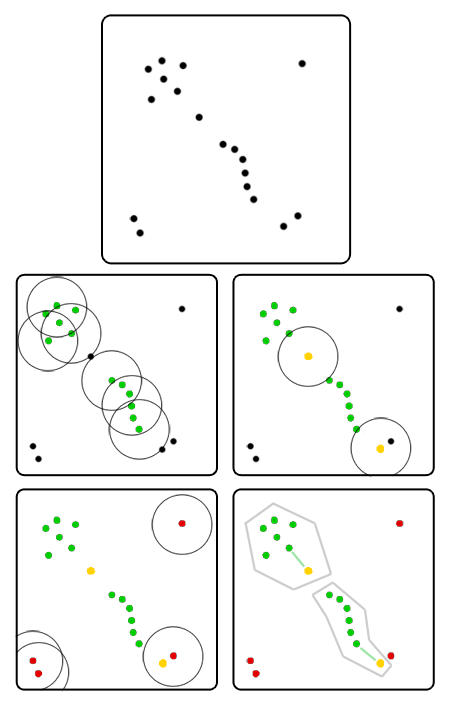
\includegraphics[scale = 1.1]{dbscan.png}
			\caption{Иллюстрация к алгоритму DBSCAN. На рисунке зелёным отмечены корневые объекты, жёлтым~---~граничные и красным~---~шумовые.}
		\end{center}
	\end{figure}
	Корневые объекты находящиеся в $\varepsilon$-окрестности друг друга объединяются в один кластер. Граничные объекты относятся к тому кластеру, к какому относится корневой
	объект, в $\varepsilon$-окрестности которого лежит данный граничный объект. Таким образом, в итоге получается разделение всех объектов на кластеры и шумовые объекты.

	\end{frame}
	
	\begin{frame}
	\frametitle{Кластеризация. Алгоритм DBSCAN}
	

	Корневые объекты находящиеся в $\varepsilon$-окрестности друг друга объединяются в один кластер. Граничные объекты относятся к тому кластеру, к какому относится корневой
	объект, в $\varepsilon$-окрестности которого лежит данный граничный объект. Таким образом, в итоге получается разделение всех объектов на кластеры и шумовые объекты.

	\end{frame}
	
	\begin{frame}
	\frametitle{Кластеризация. Алгоритм DBSCAN}
	

	\textbf{Вход:} выборка $\pmb X^{n} = \{\pmb x_1, \dots, \pmb x_{n}\}$, параметры $\varepsilon$ и $m$;
	
\textbf{Выход:} разбиение выборки на кластеры и шумовые выбросы;
\begin{enumerate}
		\item $U=X^n$, $a=0$; 
		\item \textbf{Пока} есть некластеризованные точки, т.е. $U \neq \varnothing$; 
		\item \quad взять случайную точку $\pmb x \in U$; 
		\item \quad \textbf{если} $|U_\varepsilon (\pmb x)| < m$, \textbf{то} 
		\item \quad \quad пометить $\pmb x$ как шумовой; 
		\item \quad \textbf{иначе} 
		\item \quad \quad создать новый кластер: $K=U_\varepsilon (\pmb x)$; $a = a + 1$; 
		\item \quad \quad \textbf{для всех} $\pmb x' \in K$ 
		\item \quad \quad \quad \textbf{если} $|U_\varepsilon (\pmb x')| \geq m$ \textbf{то} $K=K \cup U_\varepsilon(\pmb x')$; 
		\item \quad \quad \quad \textbf{иначе} пометить $\pmb x'$ как граничный элемент $K$; 
		\item \quad \quad соотнести объект классу $a$ для всех $\pmb x' \in K$; 
		\item \quad \quad $U=U \setminus K$ 
\end{enumerate}

	\end{frame}
	
	\begin{frame}
	\frametitle{Кластеризация. Алгоритм DBSCAN}
	

	\textbf{Достоинства:} 
\begin{itemize}
	\item Относительно быстрая кластеризация больших данных (от $O(n \ln n)$ до $O(n^2)$ в зависимости от реализации); 
	\item Позволяет обрабатыват кластеры произвольной формы (в том числе протяжённые ленты, концентрические гиперсферы); 
	\item Помимо деления на кластеры выдаёт ещё и разметку шумовых объектов; 
	\item Cам определяет количество кластеров (по модулю задания других гиперпараметров);
	\item Хорошо поддаётся модифицированию (существуют реализации, скрещенные с k-means, например). 
\end{itemize}

\textbf{Недостатки:}\\ 
	Алгоритм может неадекватно обрабатывать сильные вариации плотности данных внутри кластера, проёмы и шумовые мосты между кластерами.
	То есть метод не способен соединять кластеры через проёмы, и, наоборот, связывает явно различные кластеры через плотно населённые перемычки. Проблема особенно актуальна для данных большой размерности, так как чем больше $p$, тем больше мест, где могут случайно возникнуть проёмы или мосты.

	\end{frame}
	
	\begin{frame}
	\frametitle{Кластеризация. Оценка результата}
	

	\textbf{Среднее внутрикластерное расстояние} 
$$F_0 = \frac{\sum_{i < j}\mathbf{I}_{\{y_i = y_j\}}\rho(\pmb x_i, \pmb x_j)}{\sum_{i < j}\mathbf{I}_{\{y_i = y_j\}}},$$ 

Решая задачу кластеризации, мы хотим по возможности получать как можно более кучные кластеры, то есть минимизировать $F_0$.

	\textbf{Среднее межкластерное расстояние} 
	$$F_1 = \frac{\sum_{i < j}\mathbf{I}_{\{y_i \neq y_j\}}\rho(\pmb x_i, \pmb x_j)}{\sum_{i < j}\mathbf{I}_{\{y_i \neq y_j\}}}.$$

Среднее межкластерное расстояние, напротив, нужно максимизировать, то есть целесообразно выделять в разные кластеры наиболее удалённые друг от друга объекты.

Имеет смысл вычислять отношение пары функционалов, чтобы учесть как внутрикластерные, так и межкластерные расстояния: $F_0/F_1 \rightarrow min$.

	\end{frame}
	
		\begin{frame}
	\frametitle{Кластеризация}
	\begin{figure}[H]
	\begin{center}
		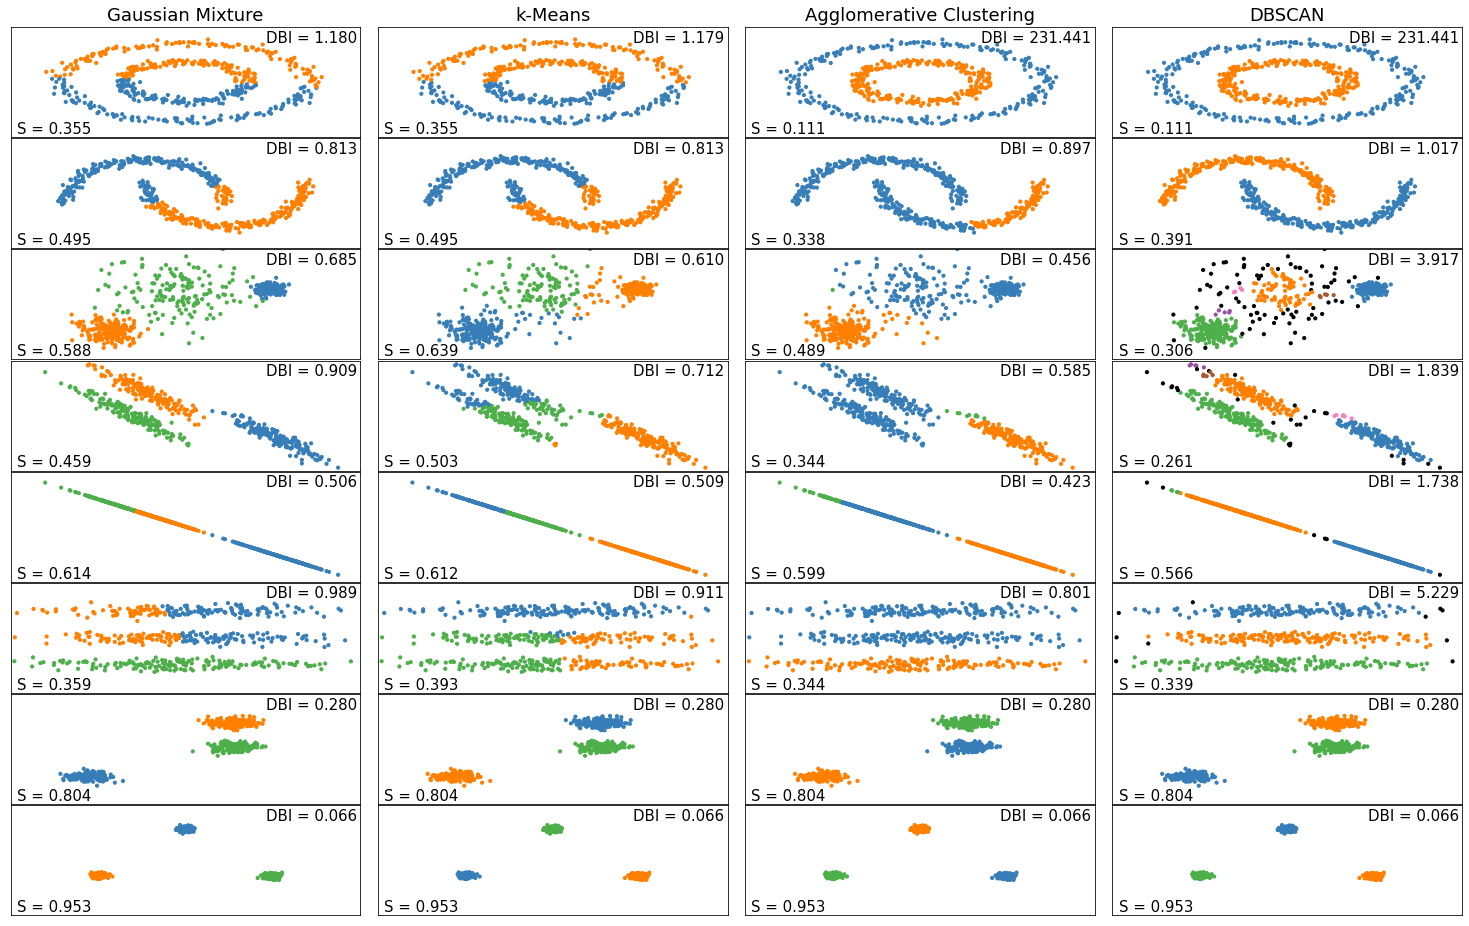
\includegraphics[scale = 0.2]{qual.png}
		\caption{Сравнение результатов работы различных алгоритмов кластеризации}
	\end{center}
\end{figure}

	\end{frame}
	
	\begin{frame}
	\frametitle{Тематическое обучение. Введение}
	Тематическое моделирование --- технология статистического анализа текстов для автоматического выявления тематики в больших коллекциях документов.
	
	Чем-то похоже на кластеризацию, но тематическое моделирование в этом плане является «мягким» и допускает, чтобы документ относился к нескольким кластерам-темам. Тематическое моделирование не претендует на понимание смысла текста, однако оно способно отвечать на вопросы «о чём этот текст» или «какие общие темы имеет эта пара текстов».
	\end{frame}
	
	\begin{frame}
	\frametitle{Тематическое обучение. Параметры тематической модели }
	

	\begin{itemize}
	\item $p(\omega | t)$  --- матрица искомых условных распределений слов по темам;
	\item $p(t | d)$ --- матрица искомых условных распределений тем по документам;
	\item $d$ --- документ;
	\item $\omega$ --- слово;
	\item $d,\omega$  --- наблюдаемые переменные;
	\item $t$  --- тема (скрытая переменная).
\end{itemize}


	\end{frame}
	
	\begin{frame}
	\frametitle{Тематическое обучение. Параметры тематической модели }
	

\begin{figure}[H]
	\begin{center}
		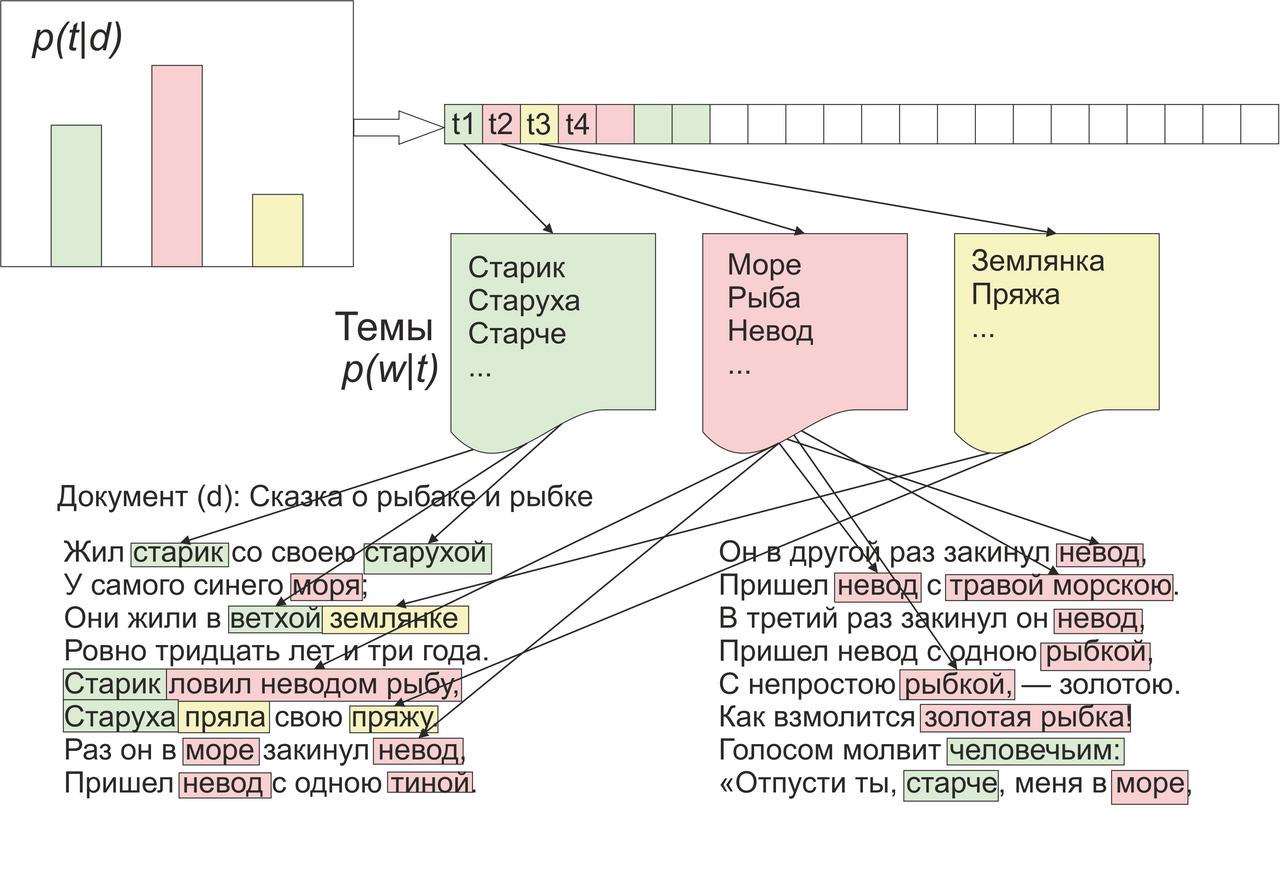
\includegraphics[scale = 1]{TM.png}
		\caption{Иллюстрация параметров модели тематического обучения.}
	\end{center}
\end{figure}
	\end{frame}
	
	\begin{frame}
	\frametitle{Тематическое обучение. LSA}
	
Латентно-семантический анализ, LSA (latent semantic analysis), он же LSI (latent semantic indexing) --- самая ранняя модель, предложенная еще в конце 80-х гг. Модель называется латентной, т.к. предполагает введение скрытого (латентного) параметра — темы.

LSA основан на использовании сингулярного разложения матрицы. С помощью SVD-разложения любая матрица раскладывается во множество ортогональных матриц, линейная комбинация которых является достаточно точным приближением к исходной матрице. Этим и объясняется название этого алгоритма в sklearn — TruncaredSVD.


	\end{frame}
	
		\begin{frame}
	\frametitle{Тематическое обучение. LSA}
	

\begin{figure}[H]
	\begin{center}
		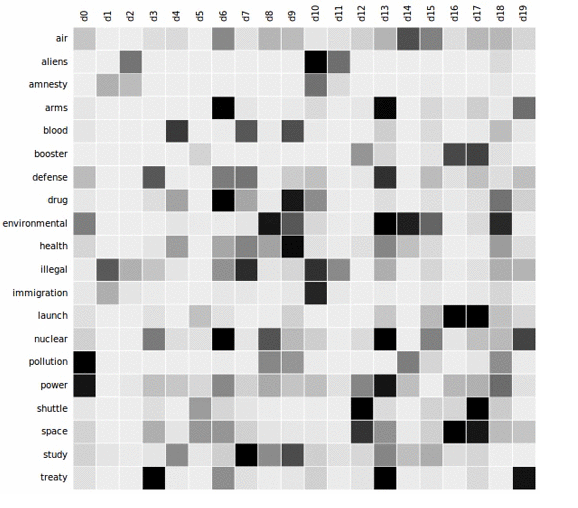
\includegraphics[scale = 0.4]{LSA1.png}
		\caption{Иллюстрация SVD в методе LSA (исходная матрица).}
	\end{center}
\end{figure}

	\end{frame}
	
			\begin{frame}
	\frametitle{Тематическое обучение. LSA}
	

\begin{figure}[H]
	\begin{center}
		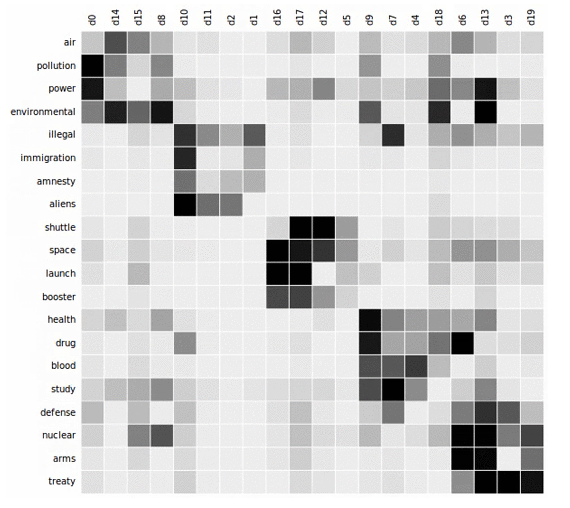
\includegraphics[scale = 0.4]{LSA2.png}
		\caption{Иллюстрация SVD в методе LSA.}
	\end{center}
\end{figure}

	\end{frame}
		\begin{frame}
	\frametitle{Тематическое обучение. pLSA}
	

pLSA (probabilistic latent semantic analysis), она же pLSI (probabilistic latent semantic indexing) --- вероятностный латентно-семантический анализ (индексирование). Модель предложена в 1999 г. Томасом Хоффманом.

Зачем понадобилось модифицировать LSA? Проблема этого метода в том, что он предполагает, что слова и документы имеют нормальное распределение, но в реальности это не так. Поэтому на практике чаще используется pLSA, основанный на мультиномиальном распределении. Если LSA — это чистая линейная алгебра, то pLSA имеет еще и статистические основания.

	\end{frame}
	
			\begin{frame}
	\frametitle{Тематическое обучение. pLSA}
	

\textbf{Дана} коллекция текстовых документов (мешок слов): $n_{d\omega}$ --- сколько раз термин $\omega$ встречаетсяя в документе $d$.

\textbf{Найти} модель $p(\omega | d) = \sum_t \phi_{\omega t}\theta_{td}$ с параметрами $\phi, \theta$:

\begin{itemize}
	\item $\phi_{\omega t} = p(\omega | t)$  --- вероятности терминов $\omega$ в каждой теме $t$;
	\item $\theta_{td} = p(t | d)$ --- вероятности тем $t$ в каждом документе $d$.
\end{itemize}

	\end{frame}
	
	\begin{frame}
	\frametitle{Тематическое обучение. pLSA}
	

Неизвестная модель находится путем максимизации логарифма правдоподобия:

$$ \sum_{d,\omega} n_{d,\omega} ln \sum_{t} \phi_{\omega t}\theta_{td} \rightarrow  \max_{\phi, \theta}$$

при ограничениях нормировки и неотрицательности:

$$ \phi_{\omega t} \geq 0; \sum_{\omega} \phi_{\omega t} = 1; \theta_{td} \geq 0; \sum_{t} \theta_{td} = 1$$

	\end{frame}
	
		\begin{frame}
	\frametitle{Тематическое обучение. pLSA}
	
Точка максимума правдоподобия $\phi, \theta$ удовлетворяет системе уравнений со вспомогательными переменными $p_{td\omega}$:
$$
\begin{cases}
\displaystyle
p_{td\omega}={ {\phi_{\omega t} \theta_{td} } \over { \sum_{t'} \phi_{\omega t'} \theta_{t'd}}}\\
\phi_{\omega t} = { {n_{\omega t}} \over {\sum_{\omega `} n_{\omega `t}}}; n_{\omega t} = \sum_{d \in D} n_{d\omega}p_{td\omega}\\
\theta_{td} = { {n_{td}} \over {\sum_{t'}n_{t'd}}}; n_{td} = \sum_{\omega \in d} n_{d\omega}p_{td\omega}
\end{cases}
$$

Где первое уравнение это $E$-шаг $EM$ алгоритма, а второе и третье уравнение --- $M$-шаг.

	\end{frame}
	
			\begin{frame}
	\frametitle{Тематическое обучение. pLSA}
	
\textbf{$E$-шаг -- это формула Байеса:}

$$p_{td\omega} = p(t | d, \omega) = { {p(\omega , t | d)} \over {p(\omega | d)}} = { {p(\omega | t) p(t|d)} \over {p(\omega | d)}}= {{\phi_{\omega t}\theta_{td}} \over {\sum_{s \in T}\phi_{\omega t}\theta_{td}}}$$

$n_{d \omega t} = n_{d \omega}p(t | d, \omega)$ --- оценка числа троек $(d, \omega, t)$ в коллекции
	\end{frame}

		\begin{frame}
	\frametitle{Тематическое обучение. pLSA}
	
\textbf{$M$-шаг --- это частотные оценки условных вероятностей:}

$$ \phi_{\omega t} = {{n_{\omega t}} \over {n_t}} \equiv {{\sum_{d \in D} n_{d \omega t}} \over {\sum_{d \in D} \sum_{\omega \in d} n_{d \omega t}}} $$

$$ \theta_{td} = { {n_td} \over {n_d}} \equiv {{\sum_{\omega \in D} n_{d \omega t}} \over {\sum_{\omega \in \Omega} \sum_{t \in T} n_{d \omega t}}}$$
	\end{frame}
	
			\begin{frame}
	\frametitle{Тематическое обучение. pLSA}
	
\textbf{Вход:} коллекция $D$, число тем $|T|$ и число иттераций $i_{max}$;
	
\textbf{Выход:} матрица терминов тем $\Theta$ и тем документов $\Phi$;

\begin{enumerate}
		\item инициализация $\phi_{\omega t}, \theta_{td}$ для всех $d \in D, \omega \in \Omega, t \in T$; 
		\item \textbf{для всех} иттераций $i=1, \cdots, i_{max}$ 
		\item \quad $n_{\omega t}, n_{td}, n_t, n_d := 0$ для всех $d \in D, \omega \in \Omega, t \in T$; 
		\item \quad \textbf{для всех} документов  $d \in D$ и слов $\omega \in d$
		\item \quad \quad $p_{td\omega} = {{\phi_{\omega t} \theta_{td}} \over {\sum_{s} \phi_{\omega s} \theta_{sd}}}$; 
		\item \quad \quad $n_{\omega t}, n_{td}, n_t, n_d += n_{d \omega} p_{td \omega}$ для всех $t \in T$;
		\item \quad $\phi_{\omega t} := n_{\omega t}/n_t$ для всех $\omega \in \Omega, t \in T$;
		\item \quad $\phi_{td} := n_{td}/n_d$ для всех $d \in D, t \in T$;

\end{enumerate}
	\end{frame}
\end{document}